\subsubsection{\stid{2.10} PROTEAS-TUNE - TAU Performance System}\label{subsubsect:tau}

\paragraph{Overview} 
The TAU Performance System is a versatile profiling and tracing toolkit that supports performance instrumentation, measurement, and analysis. It is a robust, portable, and scalable performance tool for use in parallel programs and systems over several technology generations. It is a ubiquitous performance tool suite for shared-memory and message-passing parallel applications written in C++, C, Fortran, Java, Python, UPC, and Chapel. In the PROTEAS project, TAU is being extended to support compiler-based instrumentation for the LLVM C, C++, and Fortran compilers using higher-level intermediate language representation. TAU is also targeting support for performance evaluation of directive based compilation solutions using OpenARC and it will support comprehensive performance evaluation of NVM based HPC systems.  Through these and other efforts, our objective to better support parallel runtime systems such as OpenMP, OpenACC, Kokkos, ROCm, and CUDA in TAU. Figure~\ref{figure:tau} gives an example of using TAU's parallel profile analysis tool, ParaProf.

\paragraph{Key Challenges} 
Scalable Heterogeneous Computing (SHC) platforms are gaining popularity, but it is becoming more and more complex to program these systems effectively and to evaluate their performance at scale. Performance engineering of applications must take into account multi-layered language and runtime systems, while mapping low-level actions to high-level programming abstractions.  Runtime systems such as Kokkos can shield the complexities of programming SHC systems from the programmers, but pose challenges to performance evaluation tools.  Better integration of performance technology is required.  Exposing parallelism to compilers using higher level constructs in the intermediate language provides additional opportunities for instrumentation and mapping of performance data.  It also makes possible developing new capabilities for observing multiple layers of memory hierarchy and I/O subsystems, especially for NVM-based HPC systems. 

\paragraph{Solution Strategy} Compilers and runtime systems can expose several opportunities for performance instrumentation tools such as TAU.  For instance, using the OpenACC profiling interface, TAU can tap into a wealth of information during kernel execution on accelerators as well measure data transfers between the host and devices. This can highlight when and where these data transfers occur and how long they last.  By implementing compiler-based instrumentation of LLVM compilers with TAU, it is possible to how the precise exclusive and inclusive duration of routines for programs written in C, C++, and Fortran.  Furthermore, we an take advantage of the Kokkos profiling interface to help map lower level performance data to higher level Kokkos constructs that are relevant to programmers. The instrumentation at the runtime system level can be achieved by transparently injecting the TAU Dynamic Shared Object (DSO) in the address space of the executing application. This requires no modification to the application source code or the executable. 

\begin{figure}[htb]
\centering
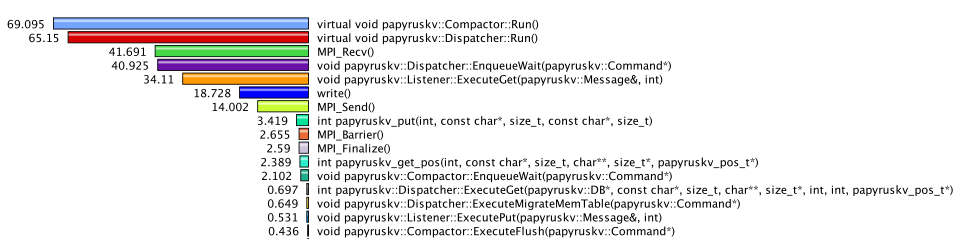
\includegraphics[width=6in]{projects/2.3.2-Tools/2.3.2.10-PROTEAS-YTUNE/tau-papyruskv}
\caption{
  Instrumentation of PapyrusKV library provides insight into asynchronous threaded library details when benchmarking 16 MPI ranks, 10k iterations with 16B keys, 1MB values on Summit using local NVM burst buffers.}
\label{figure:tau}
\end{figure}

\paragraph{Recent Progress}
\begin{enumerate}
\item \textbf{CANDLE} Extended TAU to enhance performance evaluation of multi-threaded Python3 and CUDA and applied it to evaluate the performance of the CANDLE ECP Benchmarks. TAU was extended to provide support for sampling with Python and CUDA. 

\item \textbf{Improved CUDA and OpenMP support} Updated support for CUDA and OpenCL measurement, organizing data around streams and command queues for robust multithreaded support.  Further updated the OpenMP Tools Interface support in TAU, to support the now released 5.0 standard. This OMPT v5.0 standard is currently supported in Intel v19 and Clang v8 compilers. 

\item \textbf{Flang Instrumentation} TAU support for the Flang Fortran compiler was added.  PDT- and Compiler-based instrumentation support for Flang was implemented and tested on x86\_64 Linux platforms.

\item \textbf{AMReX} TAU OpenACC measurement was demonstrated on the AMReX library.

\item \textbf{HIP} TAU's measurement library was extended to support the AMD GPU architecture. Specifically, TAU was extended to support HIP, ROCTracer, and ROCProfiler APIs under ROCm.

\item \textbf{CODAR} TAU plugin for streaming profile and trace output to ADIOS2 for realtime application monitoring.  Integrated with Chimbuko framework for runtime trace analysis, demonstrated with NWChem on Summit using 2000+ MPI ranks.

\item \textbf{NVM Measurement} Instrumented the PapyrusKV library and benchmarked performance of the library while using NVM resources on Summit.
\end{enumerate}

\paragraph{Next Steps}
\begin{enumerate}
\item \textbf{CUDA Enhancements} 
Implement new Profiling API and Perfworks Metrics API for CUDA/CUPTI 10+ to replace deprecated support for Event API and Metric API.

\item \textbf{OpenMP and OpenACC Enhancements} 
Explore and implement prototype measurement for OpenMP and OpenACC regions executed on target devices.

\item \textbf{NVM instrumentation} 
Design and implement support for supporting deep memory hierarchies in TAU for supporting MCDRAM based systems. Hardware performance counter measurements were enabled using PAPI and LIKWID toolkits.

\item \textbf{NVM Measurement} 
Added profiling and tracing support for NVM architectures.

\item \textbf{PHIRE} 
Improved LLVM IR-based selective instrumentation in TAU at the routine level using PHIRE using a TAU plugin.

\item \textbf{Outreach}
Continued outreach activities to demonstrate comprehensive performance evaluation support in TAU for OpenARC, OpenACC, LLVM compiler-based instrumentation, CUDA, Kokkos, ROCm, and NVM based programming frameworks for SHC platforms. 

\item \textbf{E4S} 
Improved integration of TAU in the E4S. 

\end{enumerate}
